\documentclass[10pt,a4paper]{article}
\usepackage[margin=1.65cm]{geometry}
\usepackage{tikz}
\usepackage[T1]{fontenc}
\usepackage[utf8]{inputenc}
\usepackage{lmodern,microtype,booktabs,tabularx,array,amsmath,enumitem,xcolor,hyperref}
\hypersetup{colorlinks=true,urlcolor=blue,linkcolor=black,pdftitle={Thesis progress update, 20 October 2026},pdfauthor={Eren Olmez}}
\setlength{\parindent}{0pt}\setlength{\parskip}{0.30em}
\setlength{\emergencystretch}{2em}
\renewcommand{\arraystretch}{1.13}
\setlist[itemize]{leftmargin=1.3em,itemsep=0.1em,topsep=0.15em}
\newcommand{\pp}{\,pp}
\newcommand{\ClassTable}{%
\begin{tabular}{@{}p{2.65cm}rp{1.65cm}p{4.0cm}p{3.75cm}@{}}
\toprule
Architecture & Overall & Worst class & Best class(es) & Median-ranked classes\\\midrule
ResNet-18 & 79.16\% & girl (45\%) & motorcycle (96\%) & kangaroo / lion (82\%)\\
ResNet-34 & 81.82\% & girl (48\%) & motorcycle (100\%) & rocket / telephone (84\%)\\
ResNet-50 & 84.39\% & girl (50\%) & chimpanzee / skunk (98\%) & hamster / leopard (86\%)\\
ResNet-101 & 85.80\% & girl (56\%) & skunk (98\%) & hamster / house (89\%)\\
MobileNetV3-Small & 62.38\% & woman (30\%) & road (93\%) & fox / telephone (62\%)\\
MobileNetV3-Large & 81.34\% & girl (50\%) & bicycle / orange / road / tractor (96\%) & house / leopard (83\%)\\
EfficientNet-B0 & 82.73\% & girl (53\%) & road / wardrobe (97\%) & table (83\%); bee (84\%)\\
ShuffleNetV2 x1.0 & 75.64\% & otter (41\%) & motorcycle (97\%) & house / poppy (76\%)\\
\bottomrule
\end{tabular}}
\newcommand{\RandomTable}{%
\begin{tabular}{@{}lrrrrrrrr@{}}
\toprule
Obj./seed & $\delta$ & Acc. Lrn & Acc. Rnd $\pm$s & $\Delta$pp & ms Lrn & ms Rnd & mJ Lrn & mJ Rnd\\\midrule
L/42 & 0.5 & 85.23$^*$ & 85.28\,$\pm$\,0.09$^*$ & -0.05 & 0.627 & 0.604 & 27.67 & 26.85\\
L/42 & 1 & 84.02$^*$ & 83.94\,$\pm$\,0.15$^*$ & +0.08 & 0.512 & 0.494 & 21.59 & 21.16\\
L/42 & 1.5 & 84.02$^*$ & 83.94\,$\pm$\,0.15$^*$ & +0.08 & 0.472 & 0.487 & 21.96 & 21.54\\
L/42 & 2 & 84.02 & 83.94\,$\pm$\,0.15 & +0.08 & 1.059 & 1.047 & 32.08 & 31.66\\
L/45 & 0.5 & 84.93$^*$ & 84.97\,$\pm$\,0.12$^*$ & -0.04 & 1.376 & 1.365 & 42.27 & 42.17\\
L/45 & 1 & 84.93 & 84.97\,$\pm$\,0.12 & -0.04 & 1.375 & 1.365 & 42.16 & 41.97\\
L/45 & 1.5 & 83.93$^*$ & 83.81\,$\pm$\,0.20$^*$ & +0.12 & 1.137 & 1.126 & 35.20 & 34.77\\
L/45 & 2 & 83.93 & 83.81\,$\pm$\,0.20 & +0.12 & 1.390 & 1.197 & 42.85 & 37.05\\
L/48 & 0.5 & 85.19$^*$ & 85.21\,$\pm$\,0.25$^*$ & -0.02 & 1.421 & 1.410 & 43.08 & 42.91\\
L/48 & 1 & 84.94 & 84.77\,$\pm$\,0.37$^*$ & +0.17 & 1.308 & 1.297 & 39.95 & 39.53\\
L/48 & 1.5 & 84.94 & 84.77\,$\pm$\,0.37 & +0.17 & 1.308 & 1.297 & 39.83 & 39.43\\
L/48 & 2 & 82.25$^*$ & 82.44\,$\pm$\,0.16$^*$ & -0.19 & 0.668 & 0.659 & 19.93 & 20.06\\
E/42 & 0.5 & 85.39 & 85.40\,$\pm$\,0.08 & -0.01 & 1.463 & 1.452 & 45.02 & 44.10\\
E/42 & 1 & 84.51$^*$ & 84.33\,$\pm$\,0.12$^*$ & +0.18 & 1.170 & 1.160 & 35.25 & 34.70\\
E/42 & 1.5 & 84.51 & 84.33\,$\pm$\,0.12 & +0.18 & 0.549 & 0.565 & 23.87 & 24.54\\
E/42 & 2 & 83.08$^*$ & 83.18\,$\pm$\,0.17$^*$ & -0.10 & 0.393 & 0.386 & 17.01 & 16.58\\
E/45 & 0.5 & 84.51$^*$ & 84.35\,$\pm$\,0.19$^*$ & +0.16 & 1.507 & 1.253 & 47.45 & 38.61\\
E/45 & 1 & 84.51$^*$ & 84.35\,$\pm$\,0.19$^*$ & +0.16 & 1.263 & 1.252 & 38.76 & 38.72\\
E/45 & 1.5 & 83.93$^*$ & 83.81\,$\pm$\,0.20$^*$ & +0.12 & 1.139 & 1.125 & 35.23 & 34.81\\
E/45 & 2 & 83.93 & 83.81\,$\pm$\,0.20 & +0.12 & 1.138 & 1.125 & 35.13 & 34.66\\
E/48 & 0.5 & 85.39 & 85.39\,$\pm$\,0.23 & +0.00 & 1.478 & 1.465 & 44.94 & 44.95\\
E/48 & 1 & 85.12 & 84.91\,$\pm$\,0.37 & +0.21 & 1.338 & 1.329 & 40.77 & 40.15\\
E/48 & 1.5 & 85.12 & 84.91\,$\pm$\,0.37 & +0.21 & 1.337 & 1.326 & 40.70 & 40.28\\
E/48 & 2 & 82.29$^*$ & 82.63\,$\pm$\,0.19$^*$ & -0.34 & 0.721 & 0.710 & 21.44 & 21.08\\
\bottomrule
\end{tabular}}
\newcommand{\UniformTable}{%
\begin{tabular}{@{}rrrr@{}}
\toprule
Seed & Uniform accuracy (\%) & ms/image & mJ/image\\\midrule
42 & 36.15 $\pm$ 2.07 & 2.072 & 55.43\\
45 & 37.28 $\pm$ 4.22 & 2.002 & 43.08\\
48 & 35.34 $\pm$ 2.57 & 1.828 & 42.98\\
\bottomrule
\end{tabular}}
\newcommand{\PrunedTable}{%
\begin{tabular}{@{}llrrrrr@{}}
\toprule
Architecture & Precision & Acc.\% & b8: ms/mJ & b32: ms/mJ & b64: ms/mJ & b128: ms/mJ\\\midrule
EfficientNet-B0 & FP32 & 14.17 & 0.407 / 17.81 & 0.135 / 6.53 & 0.124 / 5.03 & 0.101 / 4.56\\
EfficientNet-B0 & FP16 & 14.25 & 0.353 / 16.71 & 0.105 / 4.61 & 0.091 / 3.56 & 0.070 / 3.02\\
EfficientNet-B0 & INT8 & 2.33 & 0.551 / 20.75 & 0.149 / 6.44 & 0.109 / 4.13 & 0.078 / 3.32\\
MobileNetV3-Large & FP32 & 9.37 & 0.278 / 13.84 & 0.102 / 4.65 & 0.096 / 3.86 & 0.079 / 3.57\\
MobileNetV3-Large & FP16 & 9.35 & 0.249 / 10.92 & 0.085 / 3.69 & 0.069 / 2.73 & 0.054 / 2.49\\
MobileNetV3-Large & INT8 & 4.48 & 0.356 / 12.23 & 0.093 / 3.92 & 0.075 / 2.59 & 0.054 / 2.33\\
MobileNetV3-Small & FP32 & 15.49 & 0.249 / 10.22 & 0.076 / 3.12 & 0.061 / 2.20 & 0.047 / 1.93\\
MobileNetV3-Small & FP16 & 15.45 & 0.236 / 8.64 & 0.072 / 3.33 & 0.054 / 1.78 & 0.041 / 1.81\\
MobileNetV3-Small & INT8 & 4.09 & 0.330 / 10.97 & 0.091 / 3.86 & 0.061 / 2.00 & 0.041 / 1.48\\
ResNet-101 & FP32 & 2.21 & 0.337 / 16.38 & 0.194 / 8.74 & 0.183 / 8.03 & 0.154 / 7.47\\
ResNet-101 & FP16 & 2.21 & 0.285 / 13.94 & 0.102 / 5.13 & 0.103 / 4.00 & 0.085 / 3.68\\
ResNet-101 & INT8 & 2.17 & 0.369 / 15.10 & 0.112 / 4.95 & 0.094 / 3.39 & 0.071 / 2.99\\
ResNet-18 & FP32 & 3.45 & 0.181 / 8.52 & 0.124 / 5.96 & 0.126 / 5.97 & 0.112 / 5.34\\
ResNet-18 & FP16 & 3.46 & 0.120 / 5.35 & 0.069 / 3.74 & 0.075 / 2.87 & 0.064 / 2.97\\
ResNet-18 & INT8 & 3.42 & 0.117 / 5.58 & 0.056 / 2.65 & 0.057 / 2.30 & 0.047 / 2.02\\
ResNet-34 & FP32 & 3.19 & 0.218 / 10.06 & 0.139 / 6.44 & 0.136 / 6.16 & 0.116 / 5.74\\
ResNet-34 & FP16 & 3.18 & 0.146 / 6.97 & 0.076 / 3.58 & 0.073 / 2.82 & 0.060 / 2.59\\
ResNet-34 & INT8 & 3.31 & 0.187 / 8.08 & 0.072 / 3.41 & 0.065 / 2.29 & 0.054 / 2.05\\
ResNet-50 & FP32 & 3.82 & 0.250 / 10.79 & 0.146 / 7.45 & 0.148 / 6.89 & 0.128 / 6.34\\
ResNet-50 & FP16 & 3.86 & 0.185 / 8.20 & 0.087 / 4.34 & 0.087 / 3.60 & 0.073 / 3.36\\
ResNet-50 & INT8 & 2.77 & 0.223 / 9.72 & 0.082 / 3.46 & 0.069 / 2.70 & 0.057 / 2.48\\
\bottomrule
\end{tabular}}
\newcommand{\RandomProgress}{75}
\newcommand{\CutoffUTC}{2026-10-19 20:08 UTC}

\begin{document}
\begin{center}
{\Large\bfseries Thesis Progress Update}\par
{Eren Olmez}\par
{20 October 2026}\par
\end{center}
\vspace{-0.6em}
\section*{1. From scalar routing to correctness routing}
We used classical predictors with handcrafted features and lightweight convolutional neural networks (CNNs) with learned image features. Initially these predicted one scalar score; we later used 213 correctness outputs to exploit PERTINENCE's motivation: \textbf{models have complementary strengths}. Lower overall accuracy need not mean lower accuracy on every input. The target changed from one cost rank to candidate-specific success.

\textbf{Data.} Each router used a 5,000-image development pool with separate fitting/calibration subsets; 10,000 test images evaluated frozen policies. Classifiers used 45,000 training images. Deployed selection sees no test labels.

\textbf{How we calculate the scalar training score.}
\begin{enumerate}[leftmargin=1.5em,itemsep=.15em,topsep=.2em]
\item Measure candidate costs at the chosen batch size. For latency, order models from fastest to slowest; for energy, order them from least to most GPU energy. This ordering uses \emph{cost}, not accuracy.
\item For each labelled fitting image, run all candidates offline and compare their predicted classes with the true label. Mark each candidate correct or wrong.
\item Find the \emph{cheapest candidate that was correct on that image}. If its zero-based position is $r$, the training target is $s=r/(M-1)$, where $M=213$. If every candidate fails, use the reference model's position as fallback.
\item The direct batch target is the average of these per-image scores. The scalar CNN learns to predict that average using mean squared error (MSE); it does not receive the true labels at inference.
\end{enumerate}
\begin{center}\small
\begin{tabular}{@{}lccccc@{}}\toprule
Hypothetical candidates, cheapest first & A & B & C & D & E\\\midrule
Zero-based cost position &0&1&2&3&4\\
Correct on this fitting image? &No&No&Yes&Yes&No\\\bottomrule
\end{tabular}
\end{center}
C is the cheapest correct model, so this image's target is $2/(5-1)=0.50$. This is \textbf{not 50\% confidence or accuracy}. Accuracy enters through the correct/wrong labels, and later through the overall accuracy constraint.

\textbf{How the predicted score selects a model.} With the trained router fixed, calibration tries 1,601 adjustments $b\in[-1,1]$. A predicted score $z$ selects position $\operatorname{clip}(\lfloor(z+b)M\rfloor,0,M-1)$ in the cost list. For each $b$, count the selected models' correct predictions on calibration images and estimate their cost. Keep the cheapest mapping satisfying reference accuracy minus the allowance; otherwise select the reference alone. With five candidates, $z=0.46$ selects C when $b=0$ and B when $b=-0.10$. The adjustment is frozen before testing.

\begin{center}
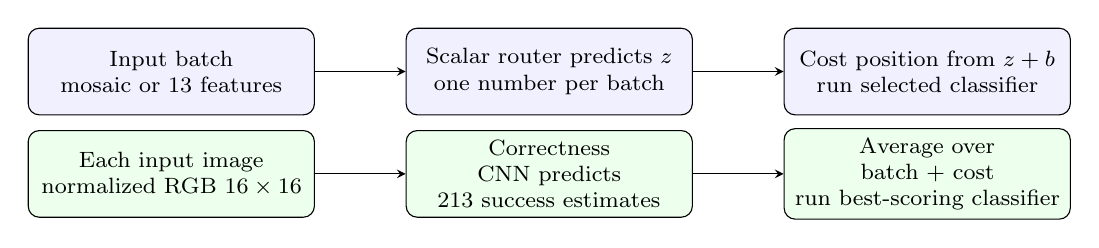
\begin{tikzpicture}[>=stealth,b/.style={draw,rounded corners,align=center,font=\footnotesize,text width=3.4cm,minimum height=11mm}]
\node[b,fill=blue!6] (a) at (0,0) {Input batch\\mosaic or 13 features};
\node[b,fill=blue!6] (b) at (4.8,0) {Scalar router predicts $z$\\one number per batch};
\node[b,fill=blue!6] (c) at (9.6,0) {Cost position from $z+b$\\run selected classifier};
\draw[->] (a)--(b);\draw[->] (b)--(c);
\node[b,fill=green!7] (d) at (0,-1.3) {Each input image\\normalized RGB $16\times16$};
\node[b,fill=green!7] (e) at (4.8,-1.3) {Correctness CNN predicts\\213 success estimates};
\node[b,fill=green!7] (f) at (9.6,-1.3) {Average over batch + cost\\run best-scoring classifier};
\draw[->] (d)--(e);\draw[->] (e)--(f);
\end{tikzpicture}
\end{center}

\textbf{Why change the target?} Wrong/right/right and wrong/right/wrong share the same cheapest-correct rank but different alternatives. Average ranks need not identify a good batch classifier. For image $x$ and candidate $m$, binary target $y_m(x)$ is 1 for correct, 0 for wrong. The CNN predicts success probability $p_m(x)$; $q_m$ is its mean over the batch. Let $C_m$ be candidate $m$'s measured latency or energy at this batch size, $C_{\max}$ the largest candidate cost, and $\lambda$ a calibrated cost penalty. Selection maximizes $q_m-\lambda C_m/C_{\max}$ over candidates. Sigmoid outputs estimate success, not CIFAR-100 classes, and need not sum to one.

\textbf{Implemented architectures and fitting.} Classical scalar inputs are 13 statistics: RGB mean/std (6), grayscale mean/std (2), gradient mean/std (2), edge density, saturation proxy and between-image brightness variation. Scalar TinyCNN uses 16 sampled $8\times8$ image tiles in a $32\times32$ mosaic: convolution $3\to16$, depthwise/pointwise $16\to24\to32\to48$, batch normalization (BN) and rectified linear activation (ReLU), global average pooling and a linear layer from 48 features to \textbf{one scalar cost-rank score per batch}. A separate calibrated mapping converts that score into a model choice. Training uses MSE, AdamW 0.001, weight decay 0.005 and 20 epochs. The correctness CNN uses each $16\times16$ image: $3\to16\to24\to32$, strided depthwise/pointwise blocks, ReLU, global pooling, 213 outputs without BN; mean binary cross-entropy, Adam 0.001, minibatches 64, 20 epochs. Three correctness fits serve seeds 42/45/48 with separate latency/energy calibration. Global scalar measurements stopped at 52 settings (stump/tree/logistic); its CNN was fitted/exported, not globally measured. The previous report completed 120 correctness-CNN settings.

\newpage
\section*{2. Why the 1.5-point results change sharply}
\textbf{The smaller model at 1.5 points is the static comparator, not necessarily the router's choice.} There are two separate decisions: the router chooses models for input batches; independently, validation chooses the cheapest eligible \emph{fixed} model as the benchmark. Savings compare these two measured costs. Accuracy allowances are percentage-point losses (pp). A stricter allowance can force the benchmark to be expensive; relaxing it can make a much faster benchmark eligible even when routing does not change.

\textbf{Exact example: latency, seed 48, batch 128.} R101/R50/R34 denote ResNet-101/50/34; FP16/FP32 mean 16/32-bit floating point; b64 means batch size 64. At both 1 and 1.5 points, routing uses R101 FP16 for 7,424 images and R34 FP16 for 2,576. It does \emph{not} switch to R50 FP16 at 1.5. R50 is the new \emph{benchmark}: its calibration accuracy loss is 1.35 pp, so it first qualifies at 1.5 points.
\begin{center}\footnotesize
\begin{tabular}{@{}rrrlrr@{}}\toprule
Allowance & Acc.\% & Route ms/mJ per image & Original benchmark & Original L\% / E\% & Fixed L\% / E\%\\\midrule
1.0&84.94&1.279 / 39.78&R101 FP16&+16.00 / +15.77&+16.00 / +15.77\\
1.5&84.94&1.277 / 39.69&R50 FP16&-47.66 / -48.21&+16.12 / +15.97\\
2.0&82.25$^*$&0.653 / 20.35&R50 FP16&+24.49 / +24.61&+57.12 / +56.92\\\bottomrule
\end{tabular}
\end{center}
\textbf{Fixed-benchmark columns:} hold the 1-point R101 FP16 benchmark at 1.52280 ms/image and 47.2306 mJ/image for all three rows. These are recalculated savings against one frozen measured reference, not new matched measurements. The 1/1.5-point savings then stay near 16\% for both costs: the large sign change in the original columns comes from the moving benchmark.
At 1.5, $100(0.865-1.277)/0.865=-47.66\%$: routing takes about 1.48 times the benchmark's time. The negative value is real underperformance against a better static alternative, not an arithmetic error. At 2 points the router favours R34 more and becomes faster, but accuracy falls below the required $85.80-2=83.80\%$ ($*$). The positive saving therefore fails the accuracy requirement.

\textbf{Why this repeats.} Across the original 120 rows, eight settings flip from positive savings at 1 point to negative at 1.5: both objectives, seed 48, batches 16/32/64/128. All eight replace R101 FP16 with R50 FP16 as benchmark. Three turn positive again at 2 points (latency b64/b128, energy b128); \emph{all three fail accuracy}. This is not a universal middle-budget anomaly: at b8 several budgets are negative throughout.

\textbf{Other large changes have a measured runtime penalty.} For latency/seed42/b8, the benchmark stays R101 FP16 from 1 to 1.5 points, but engine loads rise 217$\to$313 and evictions 215$\to$311; median routed time rises 69.46$\to$99.81 s. Calibration uses static inference costs, which omit this load/eviction overhead. A looser allowance can thus select a worse end-to-end switching pattern. Smaller residual differences between identical policies remain unexplained measurement instability; they are not evidence of an improved policy.

\section*{Why machine learning rather than scalar optimization?}
\textbf{Answer: optimization chooses the action; machine learning (ML) supplies input-specific estimates.} If only average model accuracy and cost are known, a simple constrained optimizer can select one fixed model, or fixed proportions of models, without looking at images. That is a valid baseline and does not need a neural router.

The extra question is: \emph{for this new input, which model is likely to be correct?} Global accuracy cannot answer it: a model can be best overall yet weak on forest images. A learned router tries to recognize useful input patterns before paying for a large classifier. Its success estimates then enter an ordinary numerical optimization. ML and optimization are therefore complementary, not mutually exclusive; our scalar-score router was itself an ML predictor.

\begin{center}
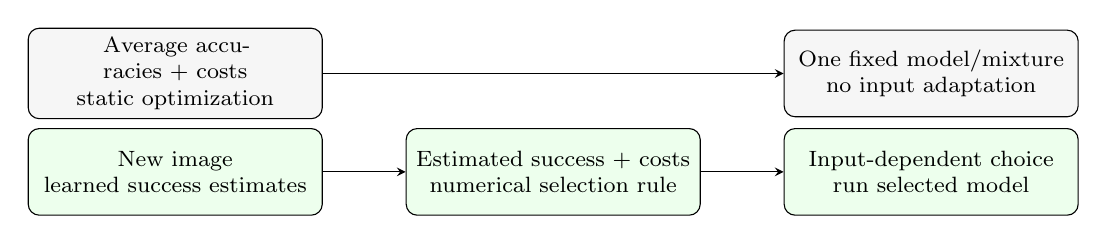
\begin{tikzpicture}[>=stealth,b/.style={draw,rounded corners,align=center,font=\footnotesize,text width=3.5cm,minimum height=11mm}]
\node[b,fill=gray!7] (a) at (0,0) {Average accuracies + costs\\static optimization};
\node[b,fill=gray!7] (b) at (9.6,0) {One fixed model/mixture\\no input adaptation};
\draw[->] (a)--(b);
\node[b,fill=green!7] (c) at (0,-1.25) {New image\\learned success estimates};
\node[b,fill=green!7] (d) at (4.8,-1.25) {Estimated success + costs\\numerical selection rule};
\node[b,fill=green!7] (e) at (9.6,-1.25) {Input-dependent choice\\run selected model};
\draw[->] (c)--(d);\draw[->] (d)--(e);
\end{tikzpicture}
\end{center}
\textbf{Justification must be empirical.} ML is useful only if better selections compensate for feature extraction, router execution and cache/loading overhead at the same required accuracy. It must beat a validation-selected static model and simple non-neural rules, not merely uniform random among weak candidates. Current results do not establish that general advantage. META-DES trained a meta-classifier to estimate candidate competence and reported improved classification accuracy against existing dynamic-selection techniques on small-sample tasks (30 classification problems in the paper). Thus learned competence estimation was useful in that study. It did not establish latency or GPU-energy savings for our CIFAR-100/TensorRT setup; those must be demonstrated by our own measurements.\footnote{Cruz et al., META-DES, \emph{Pattern Recognition}, 2015; \href{https://arxiv.org/abs/1810.01270}{author manuscript}.}

\newpage
\section*{3. Can a model be replaced without retraining the whole router?}
\textbf{Short answer.} Deletion can avoid weight retraining; unseen additions are harder. The proposed shared scorer needs initial offline training and evidence about each new model. We have not demonstrated this extension.

\textbf{Why the current router is tied to its candidates.} Its 213 outputs have fixed meanings, such as success of R101 FP16 or R34 FP16. Replacing B by B-new leaves its output predicting \emph{old B's} behaviour. Renaming the output does not teach it about B-new.

\textbf{The proposed router has three parts.} Write $x$ for an input image and $m$ for a candidate model. (1) A small \emph{image encoder}, using machine learning (ML), returns learned image features $h(x)$. (2) A \emph{shared scorer}, also ML, receives $h(x)$ and the candidate's stored profile vector $d_m$. It outputs $p_m(x)$, the estimated chance that model $m$ predicts $x$ correctly. (3) A \emph{deterministic selector}, not ML, balances these estimates against measured costs. Together they form the router; the selected CIFAR-100 classifier is downstream. A, B-new and C below are example candidate identities.

\begin{center}
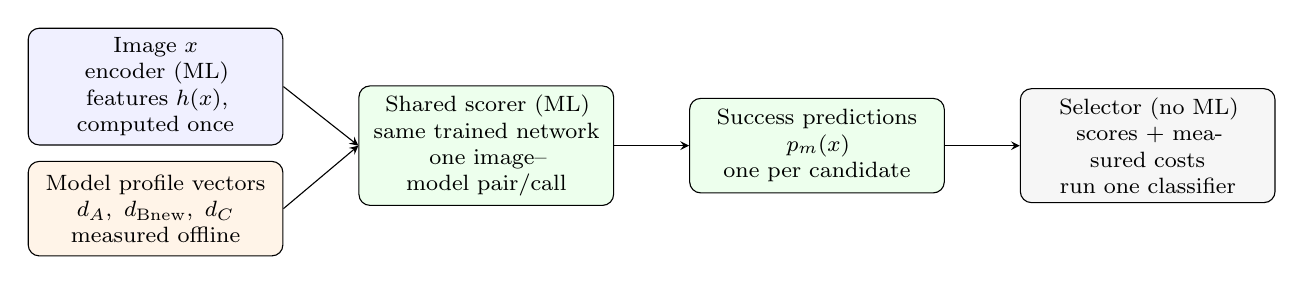
\begin{tikzpicture}[>=stealth,b/.style={draw,rounded corners,align=center,font=\footnotesize,text width=3.0cm,minimum height=12mm}]
\node[b,fill=blue!6] (a) at (0,0) {Image $x$\\encoder (ML)\\features $h(x)$, computed once};
\node[b,fill=orange!9] (b) at (0,-1.55) {Model profile vectors\\$d_A,\ d_{\rm Bnew},\ d_C$\\measured offline};
\node[b,fill=green!7] (c) at (4.2,-.75) {Shared scorer (ML)\\same trained network\\one image--model pair/call};
\node[b,fill=green!7] (d) at (8.4,-.75) {Success predictions\\$p_m(x)$\\one per candidate};
\node[b,fill=gray!7] (e) at (12.6,-.75) {Selector (no ML)\\scores + measured costs\\run one classifier};
\draw[->] (a.east)--(c.west);\draw[->] (b.east)--(c.west);\draw[->] (c)--(d);\draw[->] (d)--(e);
\end{tikzpicture}
\end{center}

\textbf{What is a model profile?} The vector $d_m$ is a numerical description with the same fields for every candidate: for example, its validation accuracy on each of the 100 classes, its precision/pruning setting and measured latency/energy. It contains no label for the current unseen image. The same format lets the scorer process a new candidate without adding a model-specific output. A profile is only a summary; class-wise accuracy alone does not reveal exactly which individual images a model gets wrong.

\textbf{How the scorer learns to produce a score.} Offline, take labelled development image $x_i$ (image number $i$) and run candidate A. If A predicts the correct class, assign $y_{iA}=1$; otherwise assign 0. Repeat for other images and candidates. The notation $[h(x_i),d_A]$ means joining the encoder's features for image $i$ with candidate A's profile; this combined vector is the scorer input. Its training target is $y_{iA}$. Fit the encoder/scorer with binary cross-entropy, using separate evidence to build profiles. Thus it learns associations between visual patterns, candidate characteristics and success. It does not calculate a reliable probability from a profile by itself, nor does it know unseen correctness.

\textbf{Inference example (hypothetical).} Suppose predicted success is A:0.70, B-new:0.85, C:0.80, with costs normalized by the largest available cost: 1.0,0.6,0.3. With penalty $\lambda=0.10$, success minus penalized cost is 0.60,0.79,0.77. B-new wins and runs on the original input. For batch routing, average each candidate's image-success estimates before selection. Feature extraction and repeated scoring must count towards runtime.

\textbf{If 50 models are removed.} The current router can mask those 50 outputs and select among 163; the proposed router instead removes 50 profile entries and scorer calls. Neither necessarily needs weight retraining for deletion. Both need policy validation/recalibration, and neither can recover accuracy if essential capabilities were removed. Deletion alone is therefore not the main advantage of the shared design.

\textbf{If a new model is added.} Evaluate it on labelled development data, measure its costs, build its profile and insert it into the registry. The existing shared scorer can accept that profile without a new head; then validate its success predictions and recalibrate selection. This is \emph{profiling/calibration}, not necessarily weight retraining, but it is still offline work. The proposed benefit is reusing the learned image--model scoring rule, rather than fitting a new named output for every replacement.

\textbf{Where this proposal comes from.} This is an adaptation of established pair-scoring and competence-estimation ideas, not a demonstrated new algorithm. Tornede et al.'s \href{https://arxiv.org/abs/2001.10741}{\emph{Extreme Algorithm Selection with Dyadic Feature Representation}} (2020) describes both problem instances and candidate algorithms using features. Our analogous pair is an image and a classifier profile. \href{https://arxiv.org/abs/1810.01270}{META-DES} learns classifier competence for a query; our proposed encoder, profiles and cost-aware single-model policy are not its original implementation.

\textbf{Deep Sets: optional extension, not required for a changing list.} Our shared scorer evaluates each candidate independently. \href{https://arxiv.org/abs/1703.06114}{Deep Sets} (Zaheer et al., NeurIPS 2017) could additionally summarize the available profiles without depending on their order, then feed that summary to the scorer. It supplies collection context, not automatic knowledge of a new model. The extra profile transformation, aggregation and scoring inputs can add computation, but latency depends on network size, caching and hardware; no overhead has been measured here. Independent scoring is the simpler first experiment because deleting B does not itself change A's correctness.

\textbf{Required validation.} Withhold entire candidate models during training, then introduce them through profiles. Test whether the frozen scorer remains accurate; otherwise fine-tune or retrain. Both designs require initial offline training and new-model profiling/calibration. Neither guarantees zero-retraining replacement, and neither has been implemented in this system.

\newpage
\section*{4. Does the learned router beat uniform random selection?}
\textbf{Answer: yes on accuracy in all 24 settings at each batch size.} At batch 64, learned accuracy is 81.86--85.64\% versus 36.26\% for uniform random; at batch 128 it is 82.25--85.39\% versus 36.25\%. Learned median latency is lower in all 24 settings at each batch; GPU energy is lower in 24/24 at batch 64 and 21/24 at batch 128. Uniform draws from all 213 candidates, including severe pruning/quantization failures. Beating it does not establish an advantage over a good static model.

\textbf{Comparison with the previous table.} Match objective, seed, batch and allowance to the 13 October correctness matrix. All 48 fresh learned accuracies equal the corresponding previous values, and fresh selection counts reproduce the frozen policies. Timings are remeasured, not copied. Each batch study comprises 495 full-test sweeps, with five trials per setting.

\begin{center}
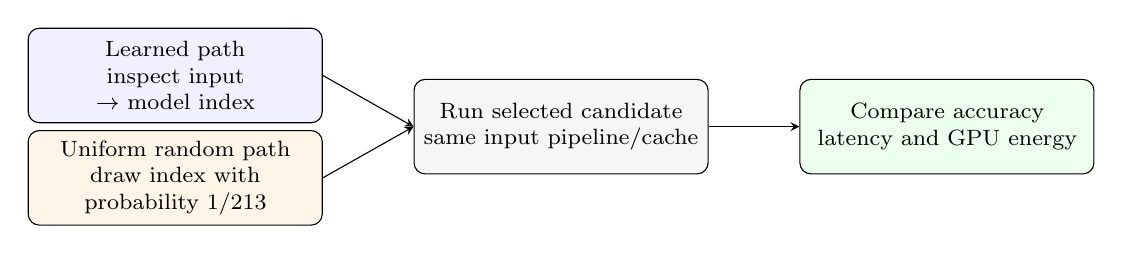
\begin{tikzpicture}[>=stealth,b/.style={draw,rounded corners,align=center,font=\footnotesize,text width=3.5cm,minimum height=12mm}]
\node[b,fill=blue!6] (a) at (0,0) {Learned path\\inspect input $\to$ model index};
\node[b,fill=orange!9] (b) at (0,-1.3) {Uniform random path\\draw index with probability $1/213$};
\node[b,fill=gray!7] (c) at (4.9,-.65) {Run selected candidate\\same input pipeline/cache};
\node[b,fill=green!7] (d) at (9.8,-.65) {Compare accuracy\\latency and GPU energy};
\draw[->] (a.east)--(c.west);\draw[->] (b.east)--(c.west);\draw[->] (c)--(d);
\end{tikzpicture}
\end{center}
\textbf{Reading the table.} ML is learned routing; R is uniform random. Accuracy columns show ML / R percentages (five-trial means). In each cost cell the pair is latency saving \% / GPU-energy saving \%, not raw costs. $\delta$ is the allowed accuracy loss in percentage points (pp); $*$ marks learned mean accuracy failing its allowance against the 85.80\% R101 FP32 reference. Every uniform row fails. L/E in Obj./seed denotes the latency/energy calibration objective.

\textbf{Savings baseline.} The Benchmark identity is the original 13 October validation-selected eligible static model, measured afresh per case. Saving is $100(C_{\rm benchmark}-C_{\rm method})/C_{\rm benchmark}$ for repeat-median latency or energy. Positive means cheaper; negative means worse. Identity is the same for the paired batch-64/128 rows, but its measured cost differs by batch and case.
\begin{center}\scriptsize\setlength{\tabcolsep}{2.0pt}\renewcommand{\arraystretch}{1.15}\begin{tabular}{@{}lrlrrrrrr@{}}
\toprule
& & & \multicolumn{3}{c}{Batch 64} & \multicolumn{3}{c}{Batch 128}\\
\cmidrule(lr){4-6}\cmidrule(l){7-9}
Obj./seed & $\delta$ & Benchmark & Acc. ML / R & ML: L / E & R: L / E & Acc. ML / R & ML: L / E & R: L / E\\\midrule
L/42 & 0.5 & R101 FP16 & 84.93$^*$ / 36.36 & +10.5 / +12.6 & -505.8 / -161.6 & 85.23$^*$ / 36.15 & +4.6 / +6.3 & -215.4 / -87.6\\
L/42 & 1 & R101 FP16 & 84.02$^*$ / 36.36 & +19.5 / +22.3 & -529.4 / -170.0 & 84.02$^*$ / 36.15 & +23.0 / +26.7 & -211.9 / -88.1\\
L/42 & 1.5 & R101 FP16 & 84.02$^*$ / 36.36 & +19.4 / +20.8 & -555.5 / -168.4 & 84.02$^*$ / 36.15 & +12.0 / +27.3 & -286.2 / -83.5\\
L/42 & 2 & R101 FP16 & 83.08$^*$ / 36.36 & +45.0 / +45.9 & -127.0 / -50.8 & 84.02 / 36.15 & +32.2 / +33.0 & -32.7 / -15.7\\
L/45 & 0.5 & R101 FP16 & 85.52 / 36.67 & +2.7 / +2.6 & -151.4 / -81.2 & 84.93$^*$ / 37.28 & +11.8 / +12.3 & -28.3 / +10.6\\
L/45 & 1 & R101 FP16 & 85.17 / 36.67 & +6.7 / +6.3 & -152.5 / -82.4 & 84.93 / 37.28 & +12.0 / +12.2 & -28.1 / +10.3\\
L/45 & 1.5 & R101 FP16 & 84.58 / 36.67 & +11.3 / +11.2 & -152.2 / -82.8 & 83.93$^*$ / 37.28 & +27.2 / +26.6 & -28.2 / +10.1\\
L/45 & 2 & R101 FP16 & 83.23$^*$ / 36.67 & +34.8 / +34.5 & -136.8 / -69.8 & 83.93 / 37.28 & +11.1 / +11.6 & -28.0 / +11.1\\
L/48 & 0.5 & R101 FP16 & 85.41 / 35.76 & +3.6 / +5.3 & -142.8 / -93.4 & 85.19$^*$ / 35.34 & +9.0 / +9.4 & -17.1 / +9.6\\
L/48 & 1 & R101 FP16 & 84.84 / 35.76 & +12.6 / +14.9 & -149.0 / -99.1 & 84.94 / 35.34 & +16.2 / +16.7 & -17.1 / +10.3\\
L/48 & 1.5 & R50 FP16 & 84.84 / 35.76 & -45.0 / -44.1 & -312.7 / -233.1 & 84.94 / 35.34 & -47.5 / -47.3 & -106.0 / -58.9\\
L/48 & 2 & R50 FP16 & 81.86$^*$ / 35.76 & +43.4 / +43.2 & -307.6 / -228.2 & 82.25$^*$ / 35.34 & +24.7 / +27.5 & -105.9 / -56.3\\
E/42 & 0.5 & R101 FP16 & 85.23$^*$ / 36.36 & +4.2 / +4.0 & -126.7 / -51.2 & 85.39 / 36.15 & +6.2 / +6.2 & -32.8 / -15.6\\
E/42 & 1 & R101 FP16 & 84.44$^*$ / 36.36 & +24.0 / +24.1 & -122.2 / -52.0 & 84.51$^*$ / 36.15 & +25.1 / +25.0 & -32.7 / -17.9\\
E/42 & 1.5 & R101 FP16 & 84.44 / 36.36 & +19.9 / +19.9 & -386.6 / -125.4 & 84.51 / 36.15 & +17.3 / +19.9 & -212.2 / -86.1\\
E/42 & 2 & R101 FP16 & 83.51$^*$ / 36.36 & -35.4 / -8.8 & -542.4 / -168.9 & 83.08$^*$ / 36.15 & +33.0 / +36.9 & -253.4 / -105.6\\
E/45 & 0.5 & R101 FP16 & 85.27$^*$ / 36.67 & +6.4 / +5.9 & -149.2 / -80.2 & 84.51$^*$ / 37.28 & +12.4 / +10.3 & -16.3 / +18.6\\
E/45 & 1 & R101 FP16 & 84.74$^*$ / 36.67 & +9.4 / +9.3 & -151.8 / -81.3 & 84.51$^*$ / 37.28 & +19.2 / +19.3 & -28.2 / +10.3\\
E/45 & 1.5 & R101 FP16 & 84.34 / 36.67 & +17.4 / +15.9 & -146.0 / -80.0 & 83.93$^*$ / 37.28 & +27.1 / +26.4 & -28.2 / +10.0\\
E/45 & 2 & R101 FP16 & 83.49$^*$ / 36.67 & +29.0 / +29.0 & -152.4 / -80.4 & 83.93 / 37.28 & +27.1 / +26.8 & -28.2 / +10.2\\
E/48 & 0.5 & R101 FP16 & 85.64 / 35.76 & +3.8 / +3.6 & -139.7 / -93.2 & 85.39 / 35.34 & +5.3 / +5.9 & -17.1 / +10.0\\
E/48 & 1 & R101 FP16 & 85.18 / 35.76 & +8.3 / +7.7 & -132.2 / -88.8 & 85.12 / 35.34 & +14.3 / +14.5 & -17.1 / +9.9\\
E/48 & 1.5 & R50 FP16 & 84.66 / 35.76 & -44.8 / -42.9 & -303.8 / -224.5 & 85.12 / 35.34 & -50.7 / -49.7 & -105.9 / -58.1\\
E/48 & 2 & R50 FP16 & 83.65$^*$ / 35.76 & -15.7 / -13.1 & -304.2 / -226.8 & 82.29$^*$ / 35.34 & +18.7 / +21.3 & -106.0 / -57.7\\
\bottomrule
\end{tabular}
\end{center}

\textbf{Shared random trials and uncertainty.} Uniform controls are reused across objectives/allowances, not independent experiments per row. For seeds 42/45/48, accuracy mean $\pm$ sample standard deviation is respectively 36.36$\pm$2.64, 36.67$\pm$1.47, 35.76$\pm$2.12\% at batch 64, and 36.15$\pm$2.07, 37.28$\pm$4.22, 35.34$\pm$2.57\% at batch 128. Different row benchmarks explain why identical random measurements can have different savings.

\textbf{Measurement boundary and caution.} Both paths include fresh GPU input preparation, selected-model load/eviction, inference and synchronization with cache capacity two. Learned routing additionally executes its CNN; random schedule generation is setup, but dispatch lookup is timed. NVIDIA reported thermal slowdown/power capping and a fixed R101 FP32 sweep varied from about 15.4 to 58 seconds. These observations prevent attributing every timing difference to routing. All accuracy failures and actual measured outcomes are retained; the policies were not retuned using these test results.

\newpage
\section*{5. Always using a fixed 90\%-pruned model}
\textbf{Answer: lower cost, but unacceptable accuracy loss.} These completed p90 controls reach 2.17--15.49\% accuracy, versus 85.80\% for unpruned R101 FP32. None meets a 0.5/1/1.5/2-pp allowance. Here p90 means the nominal 90\% pruning setting, not a guarantee of 90\% fewer operations; INT8 is 8-bit integer precision. Seven architectures, three precisions, four batches and five repeats plus references give 440 sweeps. ShuffleNet has no pruned variant.

\textbf{Comparison with 13 October.} Its correctness router reached 81.86--85.64\% across batches 64/128, far above p90. Against the same \emph{type} of fixed R101 FP32 reference, earlier routing latency/energy saving ranges were: b8 $-336.2$ to $+61.1$ / $-160.7$ to $+60.4$\%; b32 $+60.9$ to $+76.3$ / $+61.3$ to $+76.5$\%; b64 $+61.5$ to $+87.4$ / $+63.6$ to $+87.5$\%; b128 $+60.0$ to $+81.8$ / $+60.5$ to $+82.0$\%. These are separate ranges across policies, including accuracy failures, not one policy achieving every endpoint. P90 saves more cost in many rows, but sacrifices most classification accuracy.

\textbf{Savings baseline.} Table pairs are latency saving \% / GPU-energy saving \% versus fresh, same-batch R101 FP32, matching the earlier \emph{vs-FP32} definition, not the routing table's eligible-static benchmark. Accuracy is the repeat mean; costs are repeat medians. Separate sessions and observed GPU throttling limit direct cross-study timing claims.
\begin{center}\footnotesize\setlength{\tabcolsep}{3.5pt}\begin{tabular}{@{}llrrrrr@{}}
\toprule
Architecture & Precision & Acc.\% & b8: L\% / E\% & b32: L\% / E\% & b64: L\% / E\% & b128: L\% / E\%\\\midrule
EfficientNet-B0 & FP32 & 14.17 & +82.6 / +84.3 & +92.8 / +93.0 & +93.4 / +94.6 & +94.1 / +94.8\\
EfficientNet-B0 & FP16 & 14.25 & +84.9 / +85.3 & +94.4 / +95.1 & +95.1 / +96.2 & +95.9 / +96.6\\
EfficientNet-B0 & INT8 & 2.33 & +76.4 / +81.7 & +92.1 / +93.1 & +94.2 / +95.6 & +95.4 / +96.2\\
MobileNetV3-Large & FP32 & 9.37 & +88.1 / +87.8 & +94.6 / +95.0 & +94.9 / +95.8 & +95.4 / +95.9\\
MobileNetV3-Large & FP16 & 9.35 & +89.3 / +90.4 & +95.5 / +96.1 & +96.3 / +97.1 & +96.8 / +97.2\\
MobileNetV3-Large & INT8 & 4.48 & +84.7 / +89.2 & +95.0 / +95.8 & +96.0 / +97.2 & +96.8 / +97.3\\
MobileNetV3-Small & FP32 & 15.49 & +89.3 / +91.0 & +96.0 / +96.7 & +96.8 / +97.6 & +97.3 / +97.8\\
MobileNetV3-Small & FP16 & 15.45 & +89.9 / +92.4 & +96.2 / +96.4 & +97.1 / +98.1 & +97.6 / +97.9\\
MobileNetV3-Small & INT8 & 4.09 & +85.9 / +90.3 & +95.1 / +95.9 & +96.8 / +97.8 & +97.6 / +98.3\\
ResNet-101 & FP32 & 2.21 & +85.6 / +85.6 & +89.7 / +90.7 & +90.3 / +91.3 & +91.0 / +91.5\\
ResNet-101 & FP16 & 2.21 & +87.8 / +87.7 & +94.6 / +94.5 & +94.5 / +95.7 & +95.0 / +95.8\\
ResNet-101 & INT8 & 2.17 & +84.2 / +86.7 & +94.0 / +94.7 & +95.0 / +96.3 & +95.9 / +96.6\\
ResNet-18 & FP32 & 3.45 & +92.3 / +92.5 & +93.4 / +93.6 & +93.3 / +93.6 & +93.5 / +93.9\\
ResNet-18 & FP16 & 3.46 & +94.9 / +95.3 & +96.3 / +96.0 & +96.0 / +96.9 & +96.3 / +96.6\\
ResNet-18 & INT8 & 3.42 & +95.0 / +95.1 & +97.0 / +97.2 & +97.0 / +97.5 & +97.2 / +97.7\\
ResNet-34 & FP32 & 3.19 & +90.7 / +91.1 & +92.6 / +93.1 & +92.8 / +93.4 & +93.2 / +93.5\\
ResNet-34 & FP16 & 3.18 & +93.7 / +93.9 & +96.0 / +96.2 & +96.1 / +97.0 & +96.5 / +97.1\\
ResNet-34 & INT8 & 3.31 & +92.0 / +92.9 & +96.2 / +96.4 & +96.5 / +97.5 & +96.9 / +97.7\\
ResNet-50 & FP32 & 3.82 & +89.3 / +90.5 & +92.3 / +92.0 & +92.1 / +92.6 & +92.5 / +92.8\\
ResNet-50 & FP16 & 3.86 & +92.1 / +92.8 & +95.4 / +95.4 & +95.4 / +96.1 & +95.7 / +96.2\\
ResNet-50 & INT8 & 2.77 & +90.5 / +91.4 & +95.6 / +96.3 & +96.3 / +97.1 & +96.7 / +97.2\\
\bottomrule
\end{tabular}
\end{center}

% Preserve this independent class-statistics section.
\section*{6. Per-class strengths of the unpruned FP32 models}
These statistics use the entire CIFAR-100 test set: 10,000 images, balanced across 100 classes with 100 images per class. Class accuracy is the fraction of those 100 images classified correctly. Values use verified saved predictions, without new inference. All best/worst ties are shown; middle classes occupy ranks 50/51 (ties by class ID).
\begin{center}\footnotesize\renewcommand{\arraystretch}{1.22}\ClassTable\end{center}
\textbf{Complementarity example.} Forest accuracy is 62\% for R101, 71\% for R18 and 76\% for MobileNetV3-Large despite their lower overall scores. Their prior FP32 batch-32 times were 131.28, 13.64 and 6.92 ms (static boundary, not full routing). This supports PERTINENCE's motivation, not proof of routing gains; the true class is unknown at inference.\footnote{Shende et al., PERTINENCE, \emph{IEEE Access}, 2026; \href{https://doi.org/10.1109/ACCESS.2026.3707342}{paper}.}
{\footnotesize The separate 71-row supplement covers all 213 variants. Frozen numerical results/source hashes remain in \texttt{numerical\_snapshot.json}.}

\end{document}
